\chapter{Project Analysis}
\label{chap:prjan}

As discussed through Chapter ~\ref{chap:intro}, the implementation of an
ETSI-compliant MANO architecture, contemplating service chain provisioning
capabilities as mandated by RFC 7665, requires the integration of multiple
tools. The tools were chosen after their analysis, where pro and cons have been
studied and compared to the necessity of this thesis. Since the project has been
developed within the cloud environment provided by the Department of
Mathematics, University of Padua, we initially relied on Openstack (which a
product analysis can be found later in~\ref{chap:prjan:sec:openstack}) as the
default infrastructure manager choice.

\section{Available technologies in the market}
\label{chap:prjan:sec:tech}
Before starting any effective work on the project it has been decided to 
perform an analysis of the possible technologies available in the market, 
performing a choice between them and exploiting their possible ``weak 
points''. Proceeding with a top-down approach, the frameworks were chosen from 
the one that had the biggest role in the test-bed to conclude with the 
less-important components.

\subsection{Virtualized Infrastructure Manager}
A critical component, as the MANO one, is the VIM. Without it, network resources
can not be managed, and since our project was focused on dynamically allocating
containerized applications on cloud platforms, we decided to start analyzing the
right framework for this component first.

\subsubsection{Openstack}
\label{chap:prjan:sec:openstack}
Created in 2010 by a joint operation between Rackspace Hosting and
NASA~\cite{openstackWebsite}, Openstack allows on-premise cloud installations,
using bare-metal resources to provide common cloud services as object storage,
virtual machine deploy and virtual networking. Furthermore its modularity offers
the possibility to add additional components, even proprietary, to achieve a
complete cloud solution.
\begin{figure}[h]
 \centering 
\includegraphics[scale=0.58]{openstack_logo}
 \caption{Openstack logo}
 \label{chap:prjan:img:openstack_logo}
\end{figure}

\subsubsection{Kubernetes}

As already introduced before, Kubernetes is an open source software framework
specialized in container management and orchestration. Developed by Google in
2014 and written in Go~\cite{k8sGit}, it allows different machines (called nodes
from now on) to create an abstraction layer and to form a cluster where is
possible to run Docker containers without bothering about hardware constraints.
Nodes can have specific roles and specializations, all of them managed by one or
many master nodes, that actually manage the orchestration. On top of that,
Kubernetes is virtualization-agnostic, meaning that it offers the possibility to
change the virtualization software in use (i.e. from Container-based technology
to Virtual machine one).
\begin{figure}[h]
 \centering 
\includegraphics[scale=0.35]{kubernetes_logo}
 \caption{Kubernetes Logo}
 \label{chap:intro:img:k8s_logo}
\end{figure}


\subsubsection{Docker}

In recent years, with the new hardware capabilities and the recent development
of in-kernel virtualization systems (such as Hyper-V) this technology begin to
be adopted. Virtualization allows to run different systems on the same machine,
making them completely isolated and then more resilient to failures. The back of
the medal, though, is that virtual machines require large amount of resources,
especially memory, because solutions like copy-and-write of in-memory pages are
not viable anymore (since the kernel gets duplicated too), leading to
duplication of loaded libraries and assets in the memory of the host. For large
deployment containing only simple services (e.g. a back-end application serving
a website or a database) this ends up in a waste of resources. It is here that,
in 2013~\cite{dockerWebsite}, Docker was created, basing its solution on an
already existing product: Linux Container (LXC). From this framework, Docker
built an entire ecosystem, consisting in a client/server model giving the
possibility for users to simply launch, scale and delete containers (locally or
remotely with Docker-machine), a repository system where images, a layer-based
``core'' where containers start running from when they are launched, can be
stored and tagged in a sort of version control system. Finally, another couple
of solutions, called Docker-compose, and Docker Swarm have the purpose to,
respectively, orchestrate containers in a single or a clustered system.
\begin{figure}[h]
 \centering 
\includegraphics[scale=0.7]{docker_logo}
 \caption{Official Docker logo}
 \label{chap:intro:img:docker_logo}
\end{figure}

% \vspace{0.5cm}

% The development of the ETSI MANO test-bed involved the use of several 
% tecnhologies already in the market, and in some cases the creation of ad-hoc 
% solutions to solve particular issues. Here, a brief listing of the 
% well-estabilished technologies used is performed, describing even solutions 
% that at the end weren't chosen because they didn't fit with the defined goals.

\subsection{Available MANO solutions}

Another fundamental component in the architecture is the MANO, that has to
manage the Network Services and the deployment of new VNFs. Initially identified
with Openbaton (the component is described later
in~\ref{chap:prjan:sec:tech:sub:other:sub:openbaton}), afterword it has been
discovered to be not flexible enough to support other kinds of virtualization
techniques than pure or in-cloud virtual machines. Since this was a strong
project requisite that could not be easily changed, it has been decided to opt
for the creation of a smaller and simpler alternative that offered a full
integration with Docker and Kubernetes.

\subsection{Available SFC solutions}
The tools analysis revealed little about already existent VNF or NS reusable
framework implementations, so it was necessary to fill the gap. We then
developed a complete solution to create complete SFCs, trying to standardize
our vocabulary as much as possible, and giving basic documentation.

\subsection{Technologies used during development}

Since the test-bed is composed by different components and thanks to its 
modularity, the implementation of the single components has been done with the 
help of additional tools, illustrated below

\subsubsection{Docker-compose} 
Docker-compose is a tool that allows services orchestration. It automates most
of the tasks that should be performed by hand when launching one or multiple
docker containers. It is particularly useful when more containers have to
interact together, because all the services rules are described in a simple YAML
file. On top of that, it is possible to restart/stop/destroy selected services,
while keeping the other up. Additionally, it supports containers scaling and it
offers the possibility to simply get logs, interact of inspect with the defined
services. With the birth of Docker Swarm, work has started to port this tool to
the Swarm framework. At the time of this writing, the procedure to port a
Docker-compose configuration in Docker Swarm (which a description of the product
can be found in sub-section~\ref{chap:prjan:sec:tech:sub:other:sub:swarm}) it
has become completely transparent, bundling all the necessaries resources.

\begin{figure}[h]
  \centering
  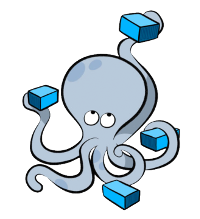
\includegraphics[scale=1]{dockercompose_logo}
  \caption[Docker-Compose logo]{Docker-Compose logo}
\end{figure}

\subsection{Other technologies evaluated}

Additional components have been evaluated during the development of the 
test-bed, and here we propose a list of the most important ones. Some of them 
where discarded as no more necessary, or during the evolution of the project 
itself they have become obsolete.

\subsubsection{Docker Swarm}
\label{chap:prjan:sec:tech:sub:other:sub:swarm}

\begin{figure}[h]
  \centering
  \includegraphics[scale=1]{dockerswarm_logo}
  \caption[Docker Swarm logo]{Docker Swarm logo}
\end{figure}

Introduced in 2014~\cite{swarmGit}, Docker Swarm allows multiple Docker nodes to
cluster together and be seen as one logical unit. This layer completely makes
the underlying infrastructure transparent: data management, as network one, are
totally managed by Docker. Recently, Docker-compose support has been introduced,
making this one-node tool available for clustered systems. At the end of the
day, on one hand Docker Swarm provides an easy way to set up a cluster system
with all the tools configured out-of-the-box, without the necessity to set
networking configurations or installing ad-hoc storage solutions. On the other
hand, though, it does not have all the customization options that Kubernetes
offers, thus making the product less flexible. This fundamental characteristic,
although, makes the two solutions have different use cases leading to different
market needs.

\subsubsection{OpenVSwitch}
Started in 2009~\cite{ovsGit}, the OpenVSwitch project aims to create an
open-source multi-layer virtual switch. It provides a switching stack for
hardware virtualization environments, implementing several interfaces and
protocols. It has also the possibility to run through Hypervisor virtualization
but it can run under Docker too~\cite{ovsDocker}. OpenVSwitch can route packets
from incoming connections following rules, that can be ``pushed'' in its routing
table from software defined as \textit{controllers}. Additionally, it supports
the OpenFlow communication protocol, in order to set previously cited routing
definitions.

\begin{figure}[h]
  \centering
  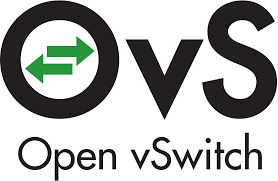
\includegraphics[scale=0.5]{ovs}
  \caption[OpenVSwitch logo]{OpenVSwitch logo}
\end{figure}

\subsubsection{Floodlight}
\label{chap:prjan:sec:tech:sub:other:sub:floodlight}
Community-developed and open source, Floodlight is an OpenFlow Controller
written in Java at the end of 2011~\cite{floodlightGit}. It allows various
applications to run on top of it. Floodlight has the role of controlling and
inquiring an OpenFlow network, querying the applications integrated with the
purpose of solving different user needs over it. When instantiated, OpenVSwitch
routers have to register to the controller in order to gain routing rules.

\begin{figure}[h]
  \centering
  
\includegraphics[scale=0.5]{floodlight_logo}
  \caption[Floodlight logo]{Floodlight logo}
\end{figure}

\subsubsection{Openbaton}
\label{chap:prjan:sec:tech:sub:other:sub:openbaton}
Patronized by the Institute Fraunhofer, it is an open-source, customizable NFV
MANO-compliant framework, that offers many configurations options, and since
it's written in Java, there is the possibility to add components (plug-ins)
dynamically. Openbaton can be installed as a normal computer program (they offer
packages for the most common distros) but it can be deployed on Docker
containers too. It is designed to work with cloud providers like Amazon or
Google Compute engine, but it offers compatibility with on-premise cloud
solutions like Openstack, where it deploys virtual machines using the API the
platform offers. It can store VNF configurations saved as Topology and
Orchestration Specification for Cloud Applications (TOSCA) Yet Another Markup
Language (YAML) and it can handle multiple Point of Presence (PoP). It offers a
VNF lifecycle management out-of-the-box, with the possibility to customize it
based on the user needs. Its modular design allows developers to change parts of
the codebase with custom ones, making the product really flexible to different
platforms. Performing this operation requires a deep knowledge of the framework
though.

\begin{figure}[h]
 \centering 
\includegraphics[scale=0.45]{openbaton_logo}
 \caption{Openbaton logo}
 \label{chap:prjan:img:openbaton_logo}
\end{figure}

\subsubsection{Dnsmasq}
\label{chap:prjan:sec:tech:sub:other:sub:dnsmasq}
Dnsmasq is an open source project, started in 2001~\cite{dnsmasqweb}. Its
features includes the possibility to serve as DNS, DHCP or router advertisement
and network boot. Dnsmasq is designed to have a small footprint memory, and it
is suited for medium to small network infrastructures. Along with the DNS
server, it has the possibility to perform request caching, to speed up
additional requests of the same type. On top of that, it provides different
compilation options in order to eliminate unused features at compile time.

\begin{figure}[h]
  \centering
  
\includegraphics[scale=0.25]{dnsmasq_logo}
  \caption{Dnsmasq logo}
\end{figure}
